\def\year{2015}
%File: formatting-instruction.tex
\documentclass[letterpaper]{article}
\usepackage{aaai}
\usepackage{times}
\usepackage{helvet}
\usepackage{courier}
\usepackage{graphicx}
\usepackage{float}
\usepackage{subfig}
\usepackage{pgfplotstable}
\usepackage{pgfplots}
\frenchspacing
\setlength{\pdfpagewidth}{8.5in}
\setlength{\pdfpageheight}{11in}
\pdfinfo{
/Title (Using Domain Knowledge to Improve Monte-Carlo Tree Search Performance in Parameterized Poker Squares)
/Author (Steven Bogaerts, Robert Arrington, Clay Langley)}
\setcounter{secnumdepth}{0}  
 \begin{document}
% The file aaai.sty is the style file for AAAI Press 
% proceedings, working notes, and technical reports.
%
\title{Using Domain Knowledge\\To Improve Monte-Carlo Tree Search Performance\\In Parameterized Poker Squares}    % ***** DON'T FORGET TO PUT TITLE IN THE METADATA ABOVE TOO!
\author{Steven Bogaerts, Robert Arrington, Clay Langley\\
Department of Computer Science\\
DePauw University\\
Greencastle, IN, USA\\
\{{\tt stevenbogaerts}, {\tt robertarrington\_2015}, {\tt claylangley\_2017}\}{\tt@depauw.edu}
}
\maketitle
\begin{abstract}
\begin{quote}
Poker Squares is a single-player card game played on a 5 x 5 grid, in which a player attempts to create as many high-scoring Poker hands as possible. As a stochastic single-player game with an extremely large state space, this game offers an interesting area of application for Monte-Carlo Tree Search (MCTS). This paper describes a variety of enhancements made to the core MCTS algorithm to improve computer play. These enhancements include hardcoding of beginning and ending moves, pruning of choice nodes in the MCTS selection stage, and a greedy MCTS simulation algorithm. The latter two enhancements make extensive use of domain knowledge in the form of a probabilistic state evaluation heuristic. Experimental results demonstrate both the general efficacy of these enhancements and their ideal parameter settings.
\end{quote}
\end{abstract}

\section{Introduction}
%Monte-Carlo Tree Search (MCTS) is a best-first search algorithm utilizing random sampling of the state space to construct a tree. Since early successes in the game of Go~\ref{*****}{\bf early Go reference here}, MCTS has garnered significant attention in the AI gaming community, with many successful applications to a variety of games~\cite{browne2012survey}.

%In the single-player card game Poker Squares, the player draws one card at a time from a standard 52-card French deck, placing each card on a 5 x 5 grid. At the end of the game, the resulting 5-card Poker hands are scored according to a given scoring system, and the player's total obtained. The game {\it Parameterized} Poker Squares (PPS) is a Poker Squares variant in which the player is given a potentially new scoring system at the start of every game. This creates an added challenge in the design of effective computer players.

Poker Squares is a single-player card game played on a 5~x~5 grid, on which the player places one drawn card at a time. Once placed, a card may not be moved. The object of the game is to create as many high-scoring Poker hands as possible in each of the five rows and five columns. Due to the overlapping of rows and columns and the uncertainty of what cards will be drawn in what order, players must balance the risk of pursuing high-scoring hands with the safer but less-rewarding pursuit of more easily-attained hands.

\begin{table}%[b]
\caption{Example scoring systems}
\label{tbl:scoring}
\centering
\begin{tabular}{c c c c c}
\hline
Hand & Am. & Brit. & F.H. & Random \\
\hline
royal flush     & 100 & 30 & -1 & -23 \\
straight flush & 75 & 30 & -1 & -55 \\
4 of a kind    & 50 & 16 & -1 & 32 \\
straight        & 25 & 10 & -1 & -64 \\
full house     & 20 & 5  & 1 & -102 \\
3 of a kind   & 15 & 12 & -1 & 16 \\
flush           & 10 & 6   & -1 & 118 \\
2 pair         & 5   & 3   & -1 & -126 \\
1 pair         & 2   & 1   & -1 & 11 \\
high card    & 0   & 0   & -1 & -128 \\
\hline
\end{tabular}
\end{table}

Two scoring systems are most common in human play: American and British. Table~\ref{tbl:scoring} lists the hand values for each. {\it Parameterized} Poker Squares (PPS) includes the added challenge that the player is not told the scoring system until the moment the game begins. So the scoring system may be standard American or British, or perhaps a system in which positive points are given for a full house and negative points for all other hands, or even a random scoring system (see Table~\ref{tbl:scoring}). Thus the player must be highly adaptive.

\begin{figure}[b]
\begin{center}
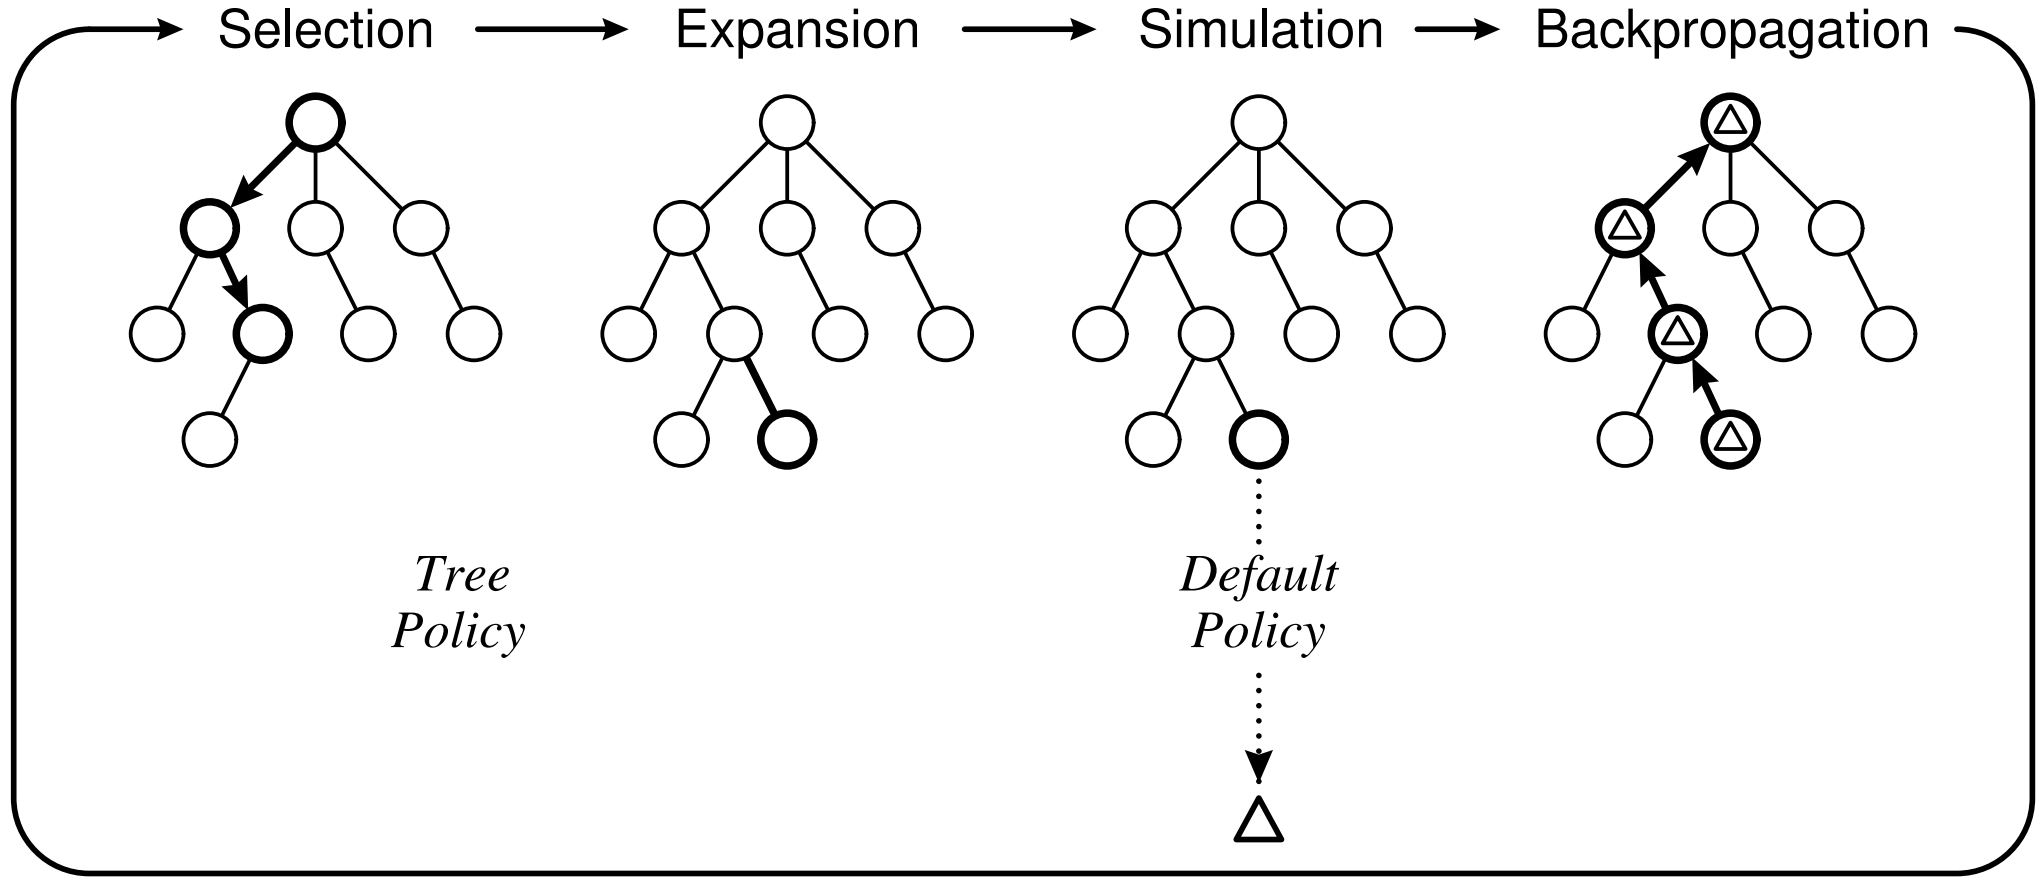
\includegraphics[width=.95\linewidth]{images/oneiteration.png}
\end{center}
\caption{Outline of MCTS~\cite{browne2012survey} }
\label{fig:OneIter}
\end{figure}

This paper considers the application of Monte-Carlo Tree Search (MCTS) to PPS. Like other game-playing algorithms, at its core MCTS involves the creation of a game tree to decide on a move. MCTS is typically applied to games with extremely large trees, because the algorithm is designed to build the tree selectively rather than exhaustively. This paper begins with a brief introduction to MCTS, followed by a discussion of related work, key enhancements to MCTS to play this game, experiments showing the effectiveness and ideal use of these enhancements, {\bf SAB what other sections will we eventually add} {\it RTA conclusions, and future work}.

\section{Monte-Carlo Tree Search}

Figure~\ref{fig:OneIter} summarizes the iterative {\it RTA was repeated} four-stage process of MCTS: selection, expansion, simulation, and backpropagation. The {\it selection} step balances goals of exploration and exploitation to select a node for further consideration. Briefly, a measure of the most ``interesting'' child of a given node is applied recursively from the root down the tree to some not-fully-expanded descendant node. One common measure of the most ``interesting'' child is the upper-confidence bound applied to trees (UCT)~\cite{kocsis2006improved}, in which a child $j$ is chosen to maximize:

\begin{equation} \label{eq:UCT}
UCT = \overline{X}_j + 2C_p\sqrt{\frac{2\ln{n}}{n_j}}
\end{equation}

\noindent where $\overline{X}_j$ is the mean score obtained in games passing through child $j$, $n$ is the number of visits to the parent node during tree construction, $n_j$ the number of visits to child $j$, and $C_p > 0$ is a constant. Thus the $\overline{X}_j$ term is the {\it exploitation} term, through which children with higher average scores will receive higher UCT scores, and therefore be more likely selected for further consideration. Similarly, the second term, {\it RTA added} $C_p$, is the {\it exploration} term, in which a child that has been visited significantly less frequently than the parent will receive a higher UCT score. Therefore, $C_p$ balances the goals of exploitation and exploration in selecting a child of a given node. Again, UCT can be applied recursively starting at the root to traverse to a not-fully-expanded node in the existing tree, thus completing the {\it selection} stage of Figure~\ref{fig:OneIter}.

Continuing in Figure~\ref{fig:OneIter}, in {\it expansion}, a previosuly unconsidered child $v$ of the selected node is randomly selected. In {\it simulation}, a game is played from $v$ to completion; in standard MCTS, simulation consists entirely of random moves. Finally, in {\it backpropagation}, the results of the simulation are used to update all nodes on the path from $v$ up to the root: each node's visit count $n$ is incremented, and each node's average score $Q$ is updated based on the result of the simulated game. In this way, the tree is gradually and selectively developed, providing an increasingly detailed picture of the expected score from various states in the state space. Upon reaching some limit condition, a child of the root can be selected based on any of a number of criteria, such as highest $Q$ or highest $n$. For a detailed discussion of the MCTS algorithm, see~\cite{browne2012survey}.

%%%%%%%%%%%%%%%%%%%%%%%%%%%%%%%%%%%%%%%%%%%%%%%%%%%%%%%%%
\section{Related Work In MCTS}

{\it RTA edits PPS is a single-player game with uncertainty while much of the MCTS research has been applied to multi-player games. Prior to MCTS these typically were attempted to be solved with a form of minimax or one of the many variations for zero-sum games which end in a win, lose, or draw. For single-player games the strategy is significantly different where a cumulative best score derived from a game's scoring rules determine a better or worse outcome, not a win or loss, but simply a higher or lower final score. {\bf SAB hmm, not entirely clear in my opinion} }

One common approach for handling uncertainty is through the use of {\it chance nodes} for the random events, in contrast to {\it choice} nodes for the player's decisions. In the selection stage of MCTS, choice nodes can be treated as usual, but chance nodes should be selected randomly rather than using UCT. We did not follow the MCTS variation as proposed by \cite{schadd2012single} which switches the position of the simulation and expansion steps for the game {\it SameGame}. However, we did find the application of a hueristic to the simulation a notable technique which we did employ. \cite{schadd2012single} did so to remove some of the randomness from what would be our chance node selection. \cite{veness2006expectimax} discusses employing chance nodes in expectimax in conjuction with the more typical maximizing and minimizing players. We understood that we did not those players types but from this dicussion in addition to the work of \cite{melko2007optimal}  and \cite{hauk2004search} we developed our player to always have choice create chance and chance to create choice nodes. {\bf SAB What's different about that approach versus what we did? Is there another paper that mentions chance nodes, and/or did something else similar to us on handling uncertainty?}

Much prior work in MCTS, as well as game-playing in general, has applied pruning to remove less-relevant branches from a game tree. In MCTS, two types of pruning are most commonly used. In {\it soft pruning}, a suboptimal node is hidden from consideration, but can brought back later if warranted by later re-evaluation. In contrast, {\it hard pruning} offers no possibility for bringing a pruned node back.~\cite{browne2012survey}. Generally the node's $Q$ value is used to determine optimality, however,  {\bf SAB Unfortunately we need to cite academic papers, not lecture notes. Do we have a paper for this?} with UCT, \cite{huang2010pruning} proposes two strategies based upon visit counts $n$: \emph{absolute pruning} all except the most visited and \emph{Relative pruning} attempts to detect when the most visited will remain so. We based or hard pruning upon $Q$ since this was holding the accumulated hand scores of the board state which carried more relevance as to the competitiveness of our player.{\bf SAB not 100\% sure what these mean, and grammar doesn't seem correct}

Additional pruning strategies using domain knowledge have been applied to the multi-player card game Lords of War~\cite{sephton2014ieee}. In this work, state evaluations based on card counting were used to prune states that were less likely to be useful. This work also considered the additional time required for such evaluations -- time that could be spent further exploring the tree. Despite this tradeoff, significant improvements were obtained with pruning based on these evaluations. We take a similar approach in this paper.

Simulation strategies enhanced with domain knowledge have also been useful in MCTS research. For example, in \cite{winands2010monte} an MCTS player for the strategy game Lines of Action used a simulation that was cut short, backpropagating a heuristic evaluation prior to the end of the game rather than playing to completion. \cite{schadd2012single} referenced earlier in their backpropogation strategy keep track of the best result so far from each node which employed in our simulation simulation when detecting for highest-scoring state so that if a trial hits that move with the decision it immediately returns it, so that future moves can have more computational time?{\bf SAB did I explain this correctly based on what you wrote? Do we have another simulation paper - especially one using a non-Random, best-move simulation like us?}

% RTA - commented
%\cite{maes2012monte} proposes a generalizable approach in the application of Monte-Carlo Search to new problems with single-player games. They suggest a language scheme for use in automatic discovery of MCTS algorithm components for use in multi-armed bandit development. By giving each element of MCTS like UCT, look-ahead, selection, and regression developed by the research of others, they define a formal method of retrieving components necessary to solve your a problem.{\bf SAB not sure what this is saying. Also, is there a connection to the work we've done?}

{\bf added by Clay} If a suitable simulation heuristic can be applied, however, the improvements to performance are significant. \cite{schadd2012single} reported a 50\% increase in average score in their player of SameGame when an accurate heuristic was added to simulation.

{\bf SAB: Anything else about domain knowledge? Maybe Cp adjustments?}

% RTA - commented
%Rather than base a pruning strategy on the visited count our focus was on estimated board score, or accumulated hand scores, at a given node which could be considered \emph{domain knowledge}. This was a hard pruning strategy because if a node was estimated to fall below a given threshold it would not be added to the tree. We had to be careful of over-pruning leaving no nodes available for selection or simulation and crashing the algorithm. This was accomplished by using a retention policy. This helped us to eliminate weaker positions and improve our player's scores.
%
%Another improvement to our player's scoring was accomplished with the implementation of a modified simulation strategy. Standard MCTS suggests choosing a child node at random and running simulations from this child. We were able to improve our scores consistently by choosing the child node with the best estimated board score.
%
%Many of the available MCTS papers discuss with varying degrees of specificity application of domain knowledge as enhancement of MCTS. Our initial implementation of the algorithm followed the model of updating $Q$ and $n$ in the \emph{backpropagation} after a simulation. $Q$ is the calculated board score of a full board of 25 cards based upon the active scoring system. With the objective of elevating our player's final game scores, we developed a system of interim board evaluation calculating an estimated hand score for each row and column containing one to four cards. Once five cards are present this value is no longer an estimate. All of the possible hand types were determined and for one to three card an a-priori probability was applied while once four cards where present then card counting was employed with it's resultant probabilities. To maintain the exploration/exploitation MCTS balance, an increasing weighting factor was applied.
%
%Some of the literature suggested positive results with multi-threading MCTS while others saw no impact. We tested a four thread player anticipating a modest increase in the number of trials accomplished. As noted by ~\cite{browne2010monte} to realize a $2X$ increase in score a $10X$ increase in the number of trials completed might be required. Our threaded player only improved on trial counts a little over $2X$ with no statistically viable improvement in score.

%%%%%%%%%%%%%%%%%%%%%%%%%%%%%%%%%%%%%%%%%%%%%%%%%%%%%%%%%
\section{MCTS Application to PPS}

%\begin{table}
%\caption{Scoring Systems: Ameritish and a random.}
%\label{tbl:SSATRD}
%\centering
%\begin{tabular}{c c c}
%\hline
%Hand & Ameritish & Random \\
%\hline
%royal flush & 47 & -23 \\
%straight flush & 47 & -55 \\
%4 of a kind & 24 & 32 \\
%straight & 13 & -64 \\
%full house & 9 & -102 \\
%3 of a kind & 8 & 16 \\
%flush & 6 & 118 \\
%2 pair & 4 & -126 \\
%1 pair & 1 & 11 \\
%high card & 0 & -128 \\
%\hline
%\end{tabular}
%\end{table}

Our MCTS application to PPS is built on top of the code in~\cite{hughart2012uct}, used under the MIT software license. The MCTS algorithm is run each time a move is needed. Thus the tree begins with a choice node at its root, in which the current card must be placed in the grid. The children are chance nodes, representing the random drawing of the next card to be played, with alternating choice and chance nodes through the remaining levels of the tree. This tree is gradually and selectively developed by repeatedly executing the four stages of MCTS as described above, with UCT in the selection stage. We limit each game to 30 seconds in total, both to make significant experimentation more manageable, and to maintain eligibility for an upcoming PPS computer player contest. 

In our ``core'' application of MCTS, the algorithm is applied to every move for an approximately equal amount of time, and domain knowledge is applied neither in selection nor in simulation. The remainder of this section will explain enhancements upon this core application of MCTS, with hard-coding certain moves and adding domain knowledge into both selection and simulation. The next section will discuss experimental results of these enhancements.

%{\bf SAB: }Pruning - remove children that are "clearly bad", but recognizing we just have an estimate, a heuristic, so not just always taking the "best", because our board evaluation is not going to be 100\% accurate, and we have uncertainty! So we need an heuristic. Lots of domain knowledge.
%5 cards: we know exactly.
%4 cards: describe the awesome stuff you guys did. 0-1-2 array, the probabilities
%1,2,3 cards: multipliers
%how 0 cards is rated
%So, with that heuristic, how is it used for pruning? Have to get at least some constant times the parent score, but then to avoid pruning everything in some cases, if below 30\% of %children, then take all above average... Pruning happens for both selection and simulation stages. Pruning only happens on choice nodes.

%{\bf SAB: }Another way to modify the system: what does simulation look like? Using the heuristic to make a decision for choice nodes, still random on chance nodes.

\subsection{Hard Coding}

%{\bf SAB: }Hardcoding of first couple and last couple moves, equivalence classes of moves

%{\bf SAB Explain briefly how this saves time.}

A brief consideration of early and late moves in PPS makes it clear that time can be saved by ``hard-coding'' certain moves with simple rules. For example, the first move is completely irrelevant. Each position in the 5~x~5 grid will be part of exactly two Poker hands, and so when the board is empty, there is no distinction between the positions. So the first card can be immediately placed arbitrarily.

For the second card, all resulting states belong in one of two equivalence classes, determined by whether or not the two cards are placed in the same hand. All other distinctions between states are irrelevant. Thus a comparatively quick calculation can be used to determine the optimal choice. {\bf SAB but we do this based on our state evaluation, don't we... Hmm. Not sure how to handle this, or if we should just gloss over it, since we haven't discussed the heuristic yet.}

Similar hard-coding can be done for the last few moves of the game. The last move, of course, is trivial, as there is only a single spot left in the grid. For two moves left, exhaustive considerations are quickly achievable.

Such processes can be continued in moves closer to the middle of the game, but they get successively more complex. In our system, we ceased hard-coding of moves with the above four policies. Thus instead of dividing 30 seconds per game among 25 moves, we can divide just under 30 seconds among the 21 remaining moves. 

\subsection{Domain Knowledge}

One benefit of the core MCTS algorithm is that very little domain knowledge is required. Nevertheless, many researchers have found great improvements with the inclusion of additional knowledge. This subsection describes a PPS state-evaluation heuristic, with the following subsections describing its application to simulation and selection.

In short, a state is evaluated by adding the scores of each of its ten Poker hands. Thus a state-evaluation heuristic is the sum of ten applications of a hand-evaluation heuristic. When the hand in question contains five cards, this is simply a matter of determining what type of Poker hand is represented, and looking up the corresponding score for the current scoring system.

For hands containing one to four cards, we first calculate a {\it possibility array}. This array contains one slot for each type of hand, from high card to royal flush. In each slot, a $0$ indicates that the hand is no longer possible, a $1$ indicates the hand is possible, and $2$ indicates the hand is already made. For example if a hand contains one card only then high card is $2$ and all of the other elements are $1$ if the single card is an ace or ten or higher otherwise the royal flush would be set to $0$. Assume the next card played into the hand produces a pair which now causes the high card element to switch to $0$ and pair becomes $2$ meaning that a score for high card is no longer possible but a pair is currently showing.{\bf SAB give an example showing this is a little trickier than people might think, like that pair gets turned off if you have 3k, etc.}.

Four-card hands use the possibility array in a different way than do one-, two-, and three-card hands. In a four-card hand, the cards remaining in the deck (those that haven't already been played) are analyzed to determine the probability that a future draw from the deck will be able to complete a ``possible'' hand (value of 1 in the array). For example, if a hand needs a 10 of hearts or 10 of clubs to complete a full house, and the remaining cards in the deck include a 10 of hearts and five different spades cards, then the probability of completing the full house is calculated as $1 / 6$. Once these probabilities are calculated for every possible hand, they can be used to obtain an expected value for the hand, by multiplying each probability by the corresponding hand value in the current scoring system.

Note that as a simplifying assumption, this calculation ignores the fact that the ten hands in the grid are dependent on each other. This dependence is due to overlap of the rows and columns on the grid, and occasional ``competition'' between hands for the same card. Nevertheless, this calculation gives a reasonable heuristic for the evaluation of four-card hands. {\bf SAB Is this all accurate? And what about a value of 2 in the array? I'm sure I'm missing some details here.}

In one-, two-, and three-card hands, this exhaustive approach proved too computationally intensive, and so some further simplifying assumptions are made. Rather than attempt to compute a probability of drawing a needed card from those remaining, we instead use {\it a-priori} probabilities of obtaining each hand in Poker Squares. We developed these a-priori probabilities from the British scoring system for Poker Squares, which is based on the difficulty of finishing each of the hands. (Note that Poker Squares probabilities are not the same as Poker probabilities.) These probabilities are then used to compute an expected value in the same way as in a four-card hand.

Note, however, that there should be some distinction between one-, two-, and three-card hands. For example, a one-card hand will have nearly all, if not all, hands listed as ``possible'' in the possibility array. A two-card hand will likely list more hands as impossible, and a three-card hand still more. Yet a three-card hand is much closer to completing its hand then a two- or one-card hand, even though all are simply listed as ``possible'' in the possibility array. So arguably, a three-card hand should be weighted more highly, all else being equal. To account for this, we apply weights $\alpha$, $\beta$, and $\gamma$ for one-, two-, and three-card hands, respectively. While we would expect that $0 < \alpha < \beta < \gamma < 1$, ideal values are the subject of an experiment described later. In an initial implementation, we fix these values at $\alpha = 0.2$, $\beta = 0.4$, and $\gamma = 0.6$.{\bf SAB fill these in. What did we do earlier experiments on? Like .2, .4, .6 or something?}

%With this, we calculated a probability for being able to finish any of the remaining possible hands in a given row or column. For example, if you had the Ten, Jack, Queen, %and King of Hearts in the topmost row, then the chance of you finishing that hand into a royal flush in the next draw is the chance of drawing the Ace of Hearts from what %remains. Alternatively, you could also finish the hand into a flush by playing any of the six Hearts cards that won’t finish the hand into a Straight or Royal flush.

It is important to point out that the above hand-evaluation calculations can readily accommodate any scoring system as a parameter. For example, if three-of-a-kind is valued at $-100$ points, then a high probability of obtaining three-of-a-kind would lead to a significant drop in expected value. Thus this heuristic allows the player to be highly adaptive to every scoring system.

\subsection{Modified Selection Through Pruning}

Recall in our core MCTS implementation that the selection process uses UCT to find a not-fully-expanded node. This means that nodes with low visit counts are favored, to some extent even when observed rewards are low. While some other games do have significantly higher branching factors than PPS, there is still potentially much to gain through pruning. The state heuristic described above can be used for this purpose.

As discussed in section {\bf (****related works****)}, there are two typical strategies for pruning: soft pruning, in which pruned nodes may be brought back, and hard pruning, in which pruned nodes are lost forever. While soft pruning may have some benefits, the decision of whether or not to bring a node back leads to extra computation and knowledge requirements, and so we opt for hard pruning in this work.

First we calculate the heuristic score for the parent, and label it $h(p)$. The value $\delta \cdot h(p)$, for some constant $\delta$, is set as the heuristic score threshold for each child. All children below this threshold are pruned, never to be considered for selection via UCT. For example, $\delta = 0.9$ would prune children with less than 90\% the score of the parent, while any $\delta > 1$ would prune all children that do not improve over the score of the parent.

In practice, this approach occasionally leads to overpruning. For example, if a card is drawn that does not fit well in any open space, all children may have lower heuristic scores than the parent. Thus an additional safeguard is put in place, that no more than 70\% of the children of any given parent may be pruned. If the  $\delta \cdot h(p)$ threshold prunes more than this amount, then only the bottom 50\% of the children are pruned.{\bf SAB Did I get this right?}

\subsection{Modified Simulation}

While the core MCTS implementation uses a completely random game in the simulation step, the state heuristic can also be applied to alternative simulation strategies. A {\it pruning simulation} strategy can apply the same pruning described above to simulation, such that a move is randomly chosen from among the non-pruned children. Alternatively, a {\it best-move simulation} can be applied, in which all children are evaluated with the state heuristic, and the highest-scoring child is taken as the choice in simulation. The tradeoff of these approaches, of course, is that they are more computationally-intensive, and thus fewer iterations of the MCTS process can be completed in a given time period. 

%%%%%%%%%%%%%%%%%%%%%%%%%%%%%%%%%%%%%%%%%%%%%%%%%%%%%%%%%
\section{Experiments and Analysis}

The modifications to the core MCTS algorithm described in the previous section are evaluated experimentally here. We begin with a discussion of the exploration-exploitation tradeoff, followed by hard-coding, and the use of domain knowledge in both simulation and selection.

%-----------------------------------------------------------------------------------------------------------------------------------------------------------------
\subsection{The Exploration--Exploitation Tradeoff}
Recall from equation (\ref{eq:UCT}) that MCTS with UCT attempts to balance the exploitation of relatively effective paths with the exploration of lesser-known paths. This balance is controlled via the constant $C_p$, where a higher value means a stronger emphasis on exploration. As discussed previously, ~\cite{kocsis2006improved} suggest that $C_p = 1 / \sqrt{2}$ is ideal when rewards range in $[0,1]$. 

In some games, using a reward range in $[0,1]$ is straightforward; for example, 0 could mean a loss, and 1 a win. Alternatively, in games with a clear maximum score, that maximum can be translated to 1, in effect ``squashing'' the scores to fit in this range.

Unfortunately, in PPS squashing to the $[0,1]$ range is not straightforward. To find the maximum score, a first attempt might be to simply take ten times the maximum-scoring hand. For example, with the American scoring system (Table~\ref{tbl:scoring}), this would be 1000. Of course it is not possible to have 10 royal flushes in a 5x5 grid, due to the dependence between hands and the use of a single deck of cards. In fact, in the American scoring system, the maximum score is 725, corresponding to four royal flushes, a straight flush, and five four-of-a-kinds. In a more unusual scoring system, a different set of hands might be higher-scoring. So it is not trivial to find the maximum score.

Compounding this problem is the difference between the maximum possible score and the most likely scores. In some scoring systems, scores close to the maximum may be somewhat easy to achieve -- for example, a scoring system in which only high-card is worth positive points. In others, however, typical scores may be far lower than the maximum possible. In the American scoring system, for example, while 725 is the maximum possible, scores in the 100s are much more common. Squashing to the $[0,1]$ range would mean that a score of 100 would become $0.138$, while a score of 150 would become $0.207$. So most scores would be in a tight range, leaving the rest of the range up to 1 rarely used. This may have unintended consequences in the UCT calculation, as nodes would look more similar than they should due to this squashing under an unrealistically high maximum possible score.

Nevertheless, we did create multiple squashing algorithms, in order to test performance with various $C_p$ values with and without squashing. The {\it precise squashing} algorithm calculates a precise minimum and maximum score in order to squash exactly to the $[0,1]$ range. Since this method is somewhat computationally intensive, a faster yet less accurate {\it imprecise squashing} method was also developed, in which the lowest possible {\it hand} score was multiplied by 10 for the minimum, and the highest hand score multiplied by 10 for the maximum. In testing the American scoring system, we also examined a simple hard-coded maximum of 200, and as a test in absurdity, another squashing method using a maximum of 2000 (2.76 times higher than the actual maximum of 725).

Each of these squashing mechanisms was tested with core MCTS by playing 700 games using the American scoring system. $C_p$ was set to $1 / \sqrt{2}$ as recommended for scores in the $[0,1]$ range. Results are shown in Table~\ref{tbl:Squashing}. The table demonstrates minimal impact of squashing accuracy; even the absurd maximum of 2000 achieved fairly comparable results. This suggests that a simple imprecise squashing method is sufficient.

\begin{table}
\captionof{table}{Effect of Score Squashing}
\label{tbl:Squashing}
\centering
\begin{tabular}{c c c}
\hline
Method & Squashing Range & Mean Score \\
\hline
Precise Squashing & 0 -- 725 & 91 \\
Imprecise Squashing & 0 -- 1000 & 91 \\
Max 200 & 0 -- 200 & 90 \\
Max 2000 & 0 -- 2000 & 90 \\
\hline
\end{tabular}
\end{table}

This begs the question, however, of whether squashing and using $C_p = 1 / \sqrt{2}$ is worthwhile at all. To explore this, we tested various $C_p$ values without squashing on the American scoring system.

As shown in  Table~\ref{tbl:noSquashing}, the lowest $C_p$ values have worse results, and at around $C_p \geq 10$ (for the American scoring system) results level off at around 92. These higher $C_p$ values mean that searches are divided as evenly as possible between not-fully-expanded nodes. Pushing $C_p$ values even higher has no further effect, even at absurd values like 10,000, because the searches are already so heavily weighted towards exploration that the node visits are distributed fairly evenly.

Note that the higher scores in Table~\ref{tbl:noSquashing} are comparable to the scores in Table~\ref{tbl:Squashing}. This is due to the similar proportions between $C_p$ and typical scores. Either $C_p  = 1 / \sqrt{2}$ and scores are in $[0,1]$, or $C_p$ and scores are both much higher. So the relative contribution of the two terms in the UCT equation (Eq.~\ref{eq:UCT}) is similar in either case.

The goal of these experiments was to fix a $C_p$ value for the experiments that follow. Table~\ref{tbl:noSquashing} suggests that, for the American scoring system, around $C_p \geq 10$ is an appopriate value to counteract the magnitude of the typical scores. Higher $C_p$ values neither increase nor decrease the mean score. Since some scoring systems will tend to have higher average scores than the American system, it is prudent to fix $C_p$ at a substantially higher value than the minimum acceptable for the American system. Thus, in future experiments, we use $C_p = 200 / \sqrt{2} = 141.4$.\footnote{This value was originally chosen based on the idea that 200 is often considered a ``winning'' score in the American system, and thus we were comparing it to a squashed value of 1. In practice this value gave good results across scoring systems, and so its use was continued, although other values would be appropriate as well.}

{\bf SAB More experiments for table 3 (Cp, no squashing, no pruning, random simulation, no calculations)}

% ***** {\bf SAB Do we want to discuss how it's better to have a higher Cp value - that some scoring systems need higher ones than others do?}

\begin{table}
\captionof{table}{Effect of $C_p$ Values With No Squashing}
\label{tbl:noSquashing}
\centering
\begin{tabular}{c c c}
\hline
$C_p$ & Mean Score \\
\hline
0 & 15 \\
$1 / \sqrt{2}$ & 64 \\
5 & 90 \\
10 & 93 \\
25 & 94 \\
50 & 93 \\
100 & 92 \\
$200 / \sqrt{2}$ & 91 \\
%1500 & 91 \\
%3000 & 93 \\
%6000 & 92 \\
10000 & 93 \\
\hline
\end{tabular}
\end{table}

%\begin{figure}
%\begin{center}
%\begin{tikzpicture}
%\begin{axis}[width=.95\linewidth,    % was axis
%	xlabel=$C_P$,
%	ylabel=Mean Score, 
%	axis lines=left,
%	%xtick={0.00, 5.00, 10.00, 25.00, 50.00},
%	xmin=0, xmax = 60,
%	ytick={30.00, 60.00,90.00,120.0},
%	ymin=0, ymax = 100,
%	scaled y ticks = false,
%	y tick label style={/pgf/number format/fixed}]
%\addplot [only marks, mark size=1pt] table[y=mean_value, x=cp]{data/cpexperiment.dat};
%\end{axis}  % was axis
%\end{tikzpicture}
%\end{center}
%\caption{$C_p$: Effect of $C_p$ on Mean Score, no Squashing.}
%\label{fig:CPEXP}
%\end{figure}

%Note - should we run more tests with different scoring systems and $C_p$ values in order to see the specificity of our current weight
%
%{\bf Note:} If we can say that our $C_p$ value should change based on the scoring system, we can go back to squashing down to 0-1 and use $1 / \sqrt{2}$, that way we can back up our decision by quoting the Brown paper and claiming to fulfill the Hoeffding inequality.
%
%If we can say that our $C_p$ value does not need to change, we would have to look more into the significance of $C_p$ values as stated by other papers, because so far other papers have said that a good $C_p$ depends heavily on the range of scores in use, so we could either dispute that or figure out why it is different for us (the chance nodes? The size of the game space? Go’s game space is even larger than ours, though I can’t recall reading about MCTS Go and $C_p$ values)

%{\bf possible tests:} run our code with a way higher (or a significantly lower) scoring system, see if it imbalances our $C_p$ value. If it does, follow up with another squashing experiment.

%{\bf SAB: May just need to say that since we didn't see a big difference in preliminary experiments, we didn't explore it further, but there could be more to explore in future work.}

%-----------------------------------------------------------------------------------------------------------------------------------------------------------------
\subsection{Hardcoding Certain Moves}

As discussed in section {\bf (****related work****)}, many researchers have found great benefit in the application of domain knowledge to MCTS. Section {\bf (****MCTS Application to parameterized poker squares****)} describes two types of domain knowledge used in PPS in this work. The first application is the implementation of hard-coded moves, in which the first two and final two moves use hard-coded rules rather than MCTS, thus allowing more time for MCTS to run in considering other moves.

%Overall, hard coding saved us 4 moves worth of time, resulting in a 19\% increase in time for each of the remaining moves over the non-hard-coded player.
%(calculation done by 4/25 = .16 ( 16\%of the total time allowed), .16/21 = .007 (each move gets an additional .7\% of the total time allowed), 1/25 = .04 (how much of the total time allowed each move gets), .007/.04 = .19 (adding the .7\% of the total time increases an individual move’s time by 19\%)

This slight increase in time for other moves led to only about a 1\% increase in score. {\bf SAB maybe we just shouldn't have this section at all, and should reduce / nearly eliminate the earlier discussion of hardcoding. It's more important to have plenty of room for the more substantial stuff. We should talk about this and figure this out as we develop other sections and see how much space we have.}

{/bf CPL I'll hold off on updating this section until we decide if it's even worth keeping}

 Allowing for other moves to have more time to run MCTS lets them make more informed decisions, but due to the very large game space the extra time given by the hard coding brings only a very small increase in performance. {\bf SAB maybe cite the paper that said you need 10 times as many trials to get twice the performance, or something?} Because hard coding saved computation time and at the very least does no harm, hard-coding remains in our final PPS implementation, but has not been explored further.

{\bf SAB we probably need to say what Cp value we're sticking with from here on out.}

{/bf CPL before saying for sure what Cp we're sticking with, I'd like to discuss the results of the overnight tests as a group. They seem strange to me, but I think if we can figure it out we can have a more optimal Cp than our current 200/rt2}

%-----------------------------------------------------------------------------------------------------------------------------------------------------------------
\subsection{Domain Knowledge and Simulation}

%fixed: Simulation improvement using domain knowledge, but no pruning in selection
%variable: totally random simulation versus just choose the best move 
%result: choose best move is better

As described above, domain knowledge has also been applied to the system via the state heuristic. This allows alternatives to the random simulation of standard MCTS. One such alternative, {\it best-move simulation}, is to use the heuristic to evaluate all children of a given node, and choose the highest-scoring child. Table~\ref{tbl:Simulate} shows the results of experimentation with this approach using the American scoring system and $C_p = 200 / \sqrt{2}$. Each row in the table is given an ID number to facilitate discussion.

Note the only difference between items (1) and (2) is whether or not heuristic calculations are done; in neither case are the calculations actually applied in simulation. Thus the drop in score from 91 to 81 demonstrates the cost of these calculations, as fewer iterations of MCTS can be achieved in a given amount of time. The 118 mean score for best-move simulation (item (3)) demonstrates that, despite the added cost of the heuristic calculations, when those calculations are actually applied to enable an enhanced simulation strategy, the added cost is worthwhile. This is consistent with what other MCTS research has shown about enhanced simulation strategies.

\begin{table}
\captionof{table}{*****What we want}
\label{tbl:Selection}
\centering
\begin{tabular}{c c c c}
\hline
ID & Sel. Method & Sim. Method & Mean Score \\
\hline
(done) & No prune calc & Random calc & 81 \\  % cost of calculations
(done) & No prune no calc & Random no calc & 91 \\ % no calculations
() & No prune no calc & best-move & \\ % (instead of (3)
() & & & \\
() & & & \\
() & & & \\



(done) & No prune no calc & Random no calc & 91 \\
() & No prune calc & Random no calc & \\
() & No prune no calc & Random calc & \\




\hline
\end{tabular}
\end{table}



\begin{table}
\captionof{table}{Effect of Domain Knowledge on Simulation}
\label{tbl:Simulate}
\centering
\begin{tabular}{c c c}
\hline
ID & Sim. Method & Mean Score \\
\hline
(1) & Random w/ Calc. & 81 \\
(2) & Random w/o Calc. & 91 \\
(3) & Best-Move & 118 \\
\hline
\end{tabular}
\end{table}

%-----------------------------------------------------------------------------------------------------------------------------------------------------------------
\subsection{Domain Knowledge and Selection}

%fixed: Pruning in selection, with just some "sensible" weights
%variable: pruning just in selection with random sim vs. pruning in selection and simulation vs. pruning in selection and choose best sim.
%result: choose best move is better, and also we see the pruning in selection is helpful
%

This set of experiments considers the application of the state heuristic to the selection step of MCTS, allowing for pruning of clearly suboptimal children. Results are shown in Table~\ref{tbl:Selection} under the American scoring system. ID numbers are continued from Table~\ref{tbl:Simulate} to facilitate comparisons.

Note that pruning selection with random simulation (item (5)) requires heuristic calculations; again, these come at a cost in fewer MCTS iterations in a given amount of time. It is important to compare the resulting mean score of 89 to the 91 in core MCTS with no calculations (item (2)). This demonstrates that pruning as designed here does not show sufficient benefit to overcome the cost of the heuristic calculations. Recall from item (3), however, that the calculations are clearly worthwhile when best-move simulation is used. So


{\bf SAB pruning is barely not worth the cost. So we should try not doing it - don't even calculate the heuristic! (but still doing best-move simulation).}



Note that selection with pruning scores show a modest increase over the core MCTS selection method, using no pruning. When combined with either of the two simulation methods discussed so far, pruning selection and best-move simulation are ideal.

{\bf SAB again, these data seem inconsistent. In Cp experiments, we have low 90's doing core MCTS (no pruning). Now with pruning we have 88.9? What's going on with these numbers? We have to figure this out before we submit the paper - this would never pass the publication review process.}

{\bf It may be beneficial to us to rework the Cp tables to use the data from the newest round of Cp experiments, the ones run this weekend. Although I am not sure why there is such a major discrepancy in score between now and our original player, at the very least we can keep all the data consistent by only using our current player edited to not perform pruning.}

\begin{table}
\captionof{table}{Effect of Domain Knowledge on Selection}
\label{tbl:Selection}
\centering
\begin{tabular}{c c c c}
\hline
ID & Sel. Method & Sim. Method & Mean Score \\
\hline
(4) & Best-Move & Best-Move & 84 \\
(5) & Pruning & Random & 89 \\
(6) & Pruning & Pruning & 107 \\
(7) & Pruning & Best-Move & 120 \\
\hline
\end{tabular}
\end{table}

{\bf SAB Clearly the calcs are good for Sim. For pruning alone, don't appear to be worth it! But already have for simulation, so can use them without any additional cost here for a little more benefit.}

Note that, while pruning selection is helpful, it does not provide as significant a jump as best-move simulation. One possible reason for this disparity is due to the number of simulations that are run compared to the number of times a node is expanded. According to our calculations, our player averages about 10 simulations per expansion. (a number given by our tracking of num pruned nodes)  Another possible reason is that, while simulations direct MCTS into which nodes are most valuable, it does not eliminate any nodes from consideration. Pruning in the expansion step, however, could potentially remove play options that aren’t actually suboptimal, due to the imprecise nature of estimated values and imperfections in our calculation.

Additionally, using our selection pruning algorithm to prune in simulation (instead of simply taking the best move) results in an increase in score over a purely random simulation step, however best-move in simulation performs better. However, best-move applied to the selection step drastically reduces the average performance. This may be because the best-move algorithm isn't perfectly calculating the best possible move every single time, however it does give the MCTS algorithm a more accurate idea of what to expect performance-wise than a pure random simulation does. This logic does not apply to the selection step, where a discounted move can never be looked at again. Pruning in selection tries to reduce the number of suboptimal moves looked at without removing the best options accidentally. Best-move in selection reduces the number of possible moves for MCTS to consider too greatly.

%-----------------------------------------------------------------------------------------------------------------------------------------------------------------
\subsection{Further Tuning of Domain Knowledge}

%fixed: pruning in selection, choose best move for simulation
%variable: the weights for the board score
%result: the best weights we came up with

 %Once we decided to keep our pruning algorithm, we ran a series of tests meant to determine what values for constants in our equation gave the best average results. When we ran tests for our potential different weights, our highest scoring test increased its score 20\% over the lowest scoring test (sheet four in our results). This shows how important an accurate method for pruning is. 

\begin{table}
\caption{Results of experiments on heuristic parameters}
\label{tbl:heuristicParameterResults}
\centering
\begin{tabular}{c c c c c c}
\hline
Mean & $\alpha$ & $\beta$ & $\gamma$ & $\beta : \alpha$ & $\gamma : \beta$\\
\hline
105.25 & 0.100 & 0.400 & 1.600 & 4.0 & 4.0 \\
109.07 & 0.050 & 0.400 & 0.600 & 8.0 & 1.5 \\
109.30 & 0.075 & 0.400 & 0.600 & 5.3 & 1.5 \\
\hline
109.89 & 0.125 & 0.400 & 0.600 & 3.2 & 1.5 \\
110.32 & 0.100 & 0.400 & 0.600 & 4.0 & 1.5 \\
111.94 & 0.500 & 0.500 & 0.700 & 1.0 & 1.4 \\
\hline
112.20 & 0.100 & 0.500 & 0.900 & 5.0 & 1.8 \\
112.81 & 0.200 & 0.500 & 0.800 & 2.5 & 1.6 \\
113.87 & 0.200 & 0.400 & 0.600 & 2.0 & 1.5 \\
\hline
114.49 & 0.300 & 0.500 & 0.700 & 1.7 & 1.4 \\
114.91 & 0.200 & 0.600 & 1.200 & 3.0 & 2.0 \\
115.14 & 0.150 & 0.450 & 1.350 & 3.0 & 3.0 \\
\hline
116.77 & 0.200 & 0.400 & 0.700 & 2.0 & 1.8 \\
116.95 & 0.125 & 0.250 & 0.500 & 2.0 & 2.0 \\
117.37 & 0.200 & 0.500 & 0.900 & 2.5 & 1.8 \\
\hline
118.72 & 0.050 & 0.200 & 0.800 & 4.0 & 4.0 \\
118.79 & 0.150 & 0.300 & 0.900 & 2.0 & 3.0 \\
119.42 & 0.050 & 0.150 & 0.450 & 3.0 & 3.0 \\
\hline
119.50 & 0.125 & 0.250 & 0.750 & 2.0 & 3.0 \\
119.66 & 0.200 & 0.400 & 0.900 & 2.0 & 2.3 \\
119.95 & 0.100 & 0.300 & 0.700 & 3.0 & 2.3 \\
\hline
119.99 & 0.150 & 0.300 & 0.600 & 2.0 & 2.0 \\
120.58 & 0.100 & 0.300 & 0.750 & 3.0 & 2.5 \\
120.75 & 0.100 & 0.200 & 0.750 & 2.0 & 3.8 \\
\hline
121.14 & 0.094 & 0.283 & 0.850 & 3.0 & 3.0 \\
121.60 & 0.075 & 0.150 & 0.500 & 2.0 & 3.3 \\
121.68 & 0.100 & 0.300 & 0.800 & 3.0 & 2.7 \\
\hline
121.99 & 0.100 & 0.300 & 0.900 & 3.0 & 3.0 \\
123.21 & 0.100 & 0.300 & 0.850 & 3.0 & 2.8 \\
\hline
\end{tabular}
\end{table}

\begin{figure}
\begin{center}
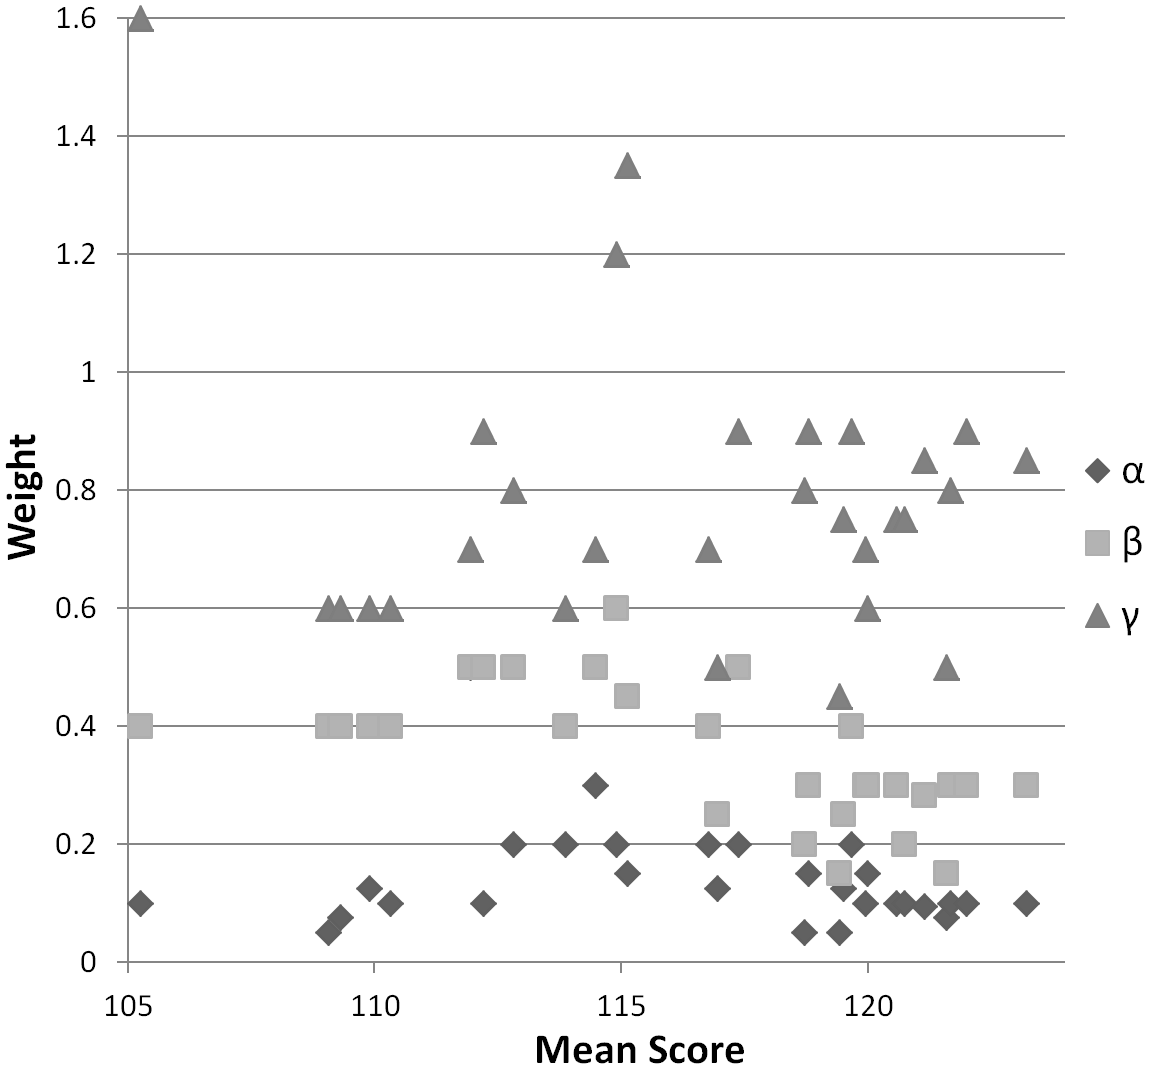
\includegraphics[width=1\linewidth]{images/1-2-3_weights.png}
\end{center}
\caption{$\alpha$, $\beta$, and $\gamma$ for each resulting mean score.}
\label{fig:123weights}
\end{figure}

\begin{figure}
\begin{center}
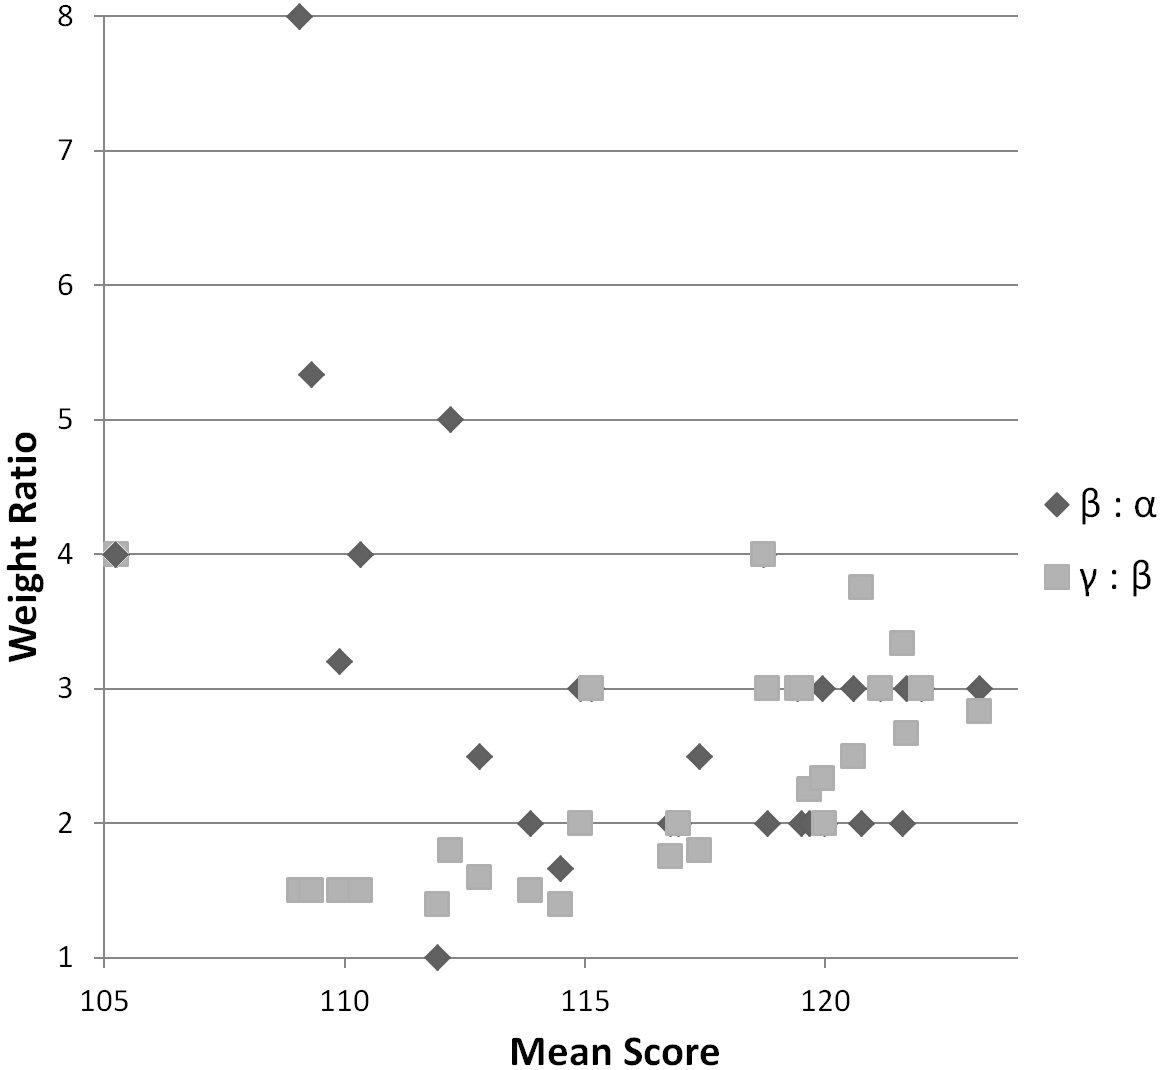
\includegraphics[width=1\linewidth]{images/1-2-3_ratios.png}
\end{center}
\caption{$\beta:\alpha$ and $\gamma:\beta$ for each resulting mean score.}
\label{fig:123ratios}
\end{figure}

The experimental results described so far show that some modifications have a very small effect, while others have a more significant effect. Recall in the discussion of the state heuristic that it includes parameters $\alpha$, $\beta$, and $\gamma$ for the weighting given to one-, two-, and three-card hands, respectively. Prior experiments used a ``reasonable'' guess for these parameters. In this experiment, we examine these parameters more closely, with the system fixed at a $C_p$ value of {\bf SAB Cp value used here *****}, hardcoding of starting and ending moves, pruning selection, and best-move simulation. These represent the best design decisions resulting from the previous experiments. The parameter settings considered here have an influence on both the selection and simulation steps, as both depend on the heuristic.

Twenty-nine different trials were conducted for various settings of the parameters, with each trial involving several hours of game play. A few intuitive ideas were used to constrain the number of permutations considered. First, we ensured that $\alpha \leq \beta \leq \gamma$, since all else being equal, a hand with more cards is closer to completing any potential hands than one with fewer cards, and so it should be valued more highly. Second, the parameter space can be constrained somewhat by considering the ratios $\beta : \alpha$ and $\gamma : \beta$. This can bring new insights into what parameter settings may be more similar than would first appear by considering magnitudes alone, thus leading to hypotheses about what portions of the space should be prioritized for consideration. Having said this, however, recall that four-card hands are evaluated using an entirely different formula. So in fact the magnitudes of $\alpha$, $\beta$, and $\gamma$ do matter as well, rather than just the ratios, because hands with three or fewer cards will be compared not just among themselves but against four- and even five-card hands. So using ratios can be a useful analysis tool, but should not be used to the exclusion of considerations of magnitude.

Results of these experiments are shown in Table~\ref{tbl:heuristicParameterResults} and in Figures~\ref{fig:123weights} and \ref{fig:123ratios}, with the table showing the raw data used to generate the figures. Note that the table is sorted in order of increasing mean score, with values ranging from 105.25 to 123.21. For each mean score, the $\alpha$, $\beta$, and $\gamma$ values and the $\beta : \alpha$ and $\gamma : \beta$ ratios are provided. Visualization is challenging due to the presence of three independent variables, but some important insights can be gained from Figures~\ref{fig:123weights} and \ref{fig:123ratios}. In both graphs, note that the horizontal axis is the mean score, and vertical axis is the weight. Thus, the three shapes on the far left in Figure~\ref{fig:123weights} correspond to the values of $\alpha$, $\beta$, and $\gamma$ in the first row of the table. These are the parameter settings that led to a mean score of 105.25.

Note in both graphs that the results are fairly scattered on the left side where mean scores are lower, yet somewhat more uniform on the right side where mean scores are higher. This demonstrates a preference for certain parameter settings to obtain the highest scores. For example, in Figure~\ref{fig:123weights}, not only the single highest-scoring player, but nearly all higher-scoring players tend to have values around $\alpha = 0.1$, $\beta = 0.3$, and $\gamma = 0.85$, with stronger convergence in the $\alpha$ and $\beta$ values.

Figure~\ref{fig:123ratios} shows ratios. Recall that ratios are harder to work with because they ignore the magnitudes of the parameters, and thus the convergence is not quite as clear as in the parameter values themselves. Nevertheless a trend is visible, in which both a $\beta : \alpha$ ratio and $\gamma : \beta$ ratio of 2 or 3 is found in the highest-scoring players. Note that these ratios correspond well to the ideal parameter values already mentioned.

{\bf SAB But we have more experiments here too, right? Some that ran for an extra long time, and some on the 4-card weight. What important conclusions could we draw from those if we wrote them up carefully?}

{\bf SAB ***** Make sure we address the different scoring systems - does system perform well with them?}

{\bf CPL addressed in the Cp section}

{\bf SAB Maybe a section about broader conclusions to draw... (not just in PPS)}

%%%%%%%%%%%%%%%%%%%%%%%%%%%%%%%%%%%%%%%%%%%%%%%%%%%%%%%%%
\section{Future Work}

{\bf SAB Might have room for a section like this........}

The size of our game space is calculated as $\frac{52!}{27\times26}$ or $1.12 \times 10^{65}$. MCTS constructs very large trees and as surveyed in~\cite{browne2012survey} may be well suited to parallelization and\/or multi-threading. Several techniques are possible such as parallel tree simulation where multiple trees are processed simultaneously. A possible drawback to this approach is that since each thread uses a copy of the same tree they may traverse similar or even identical parts of the tree. Root parallelization initiates each thread with the same beginning root but then builds independant trees. A possible advantage here is that each thread may run to a limit and stop at any time idependantly.

%%%%%%%%%%%%%%%%%%%%%%%%%%%%%%%%%%%%%%%%%%%%%%%%%%%%%%%%%

\section{whatevs}

Now we step back and look at bigger picture conclusions from the results, and theorize about why certain things were more effective than others.

Size of the game space in Poker Squares - 

Conclusion 1 - Continuing the tree search if the most visited root is not also the one with the highest reward has proven effective in some MCTS algorithms like the GO program ERICA (MCTS survey pg 8). However, this approach did nothing for our average score. We believe this to be because continuing to run MCTS on one move would take time away from subsequent moves, and due to our short amount of time with which to play this game reducing the time of later moves counteracted the benefit of continuing the search.

Conclusion 2 - Hard coding of moves. Some moves in Poker Squares can boil down to very straightforward decisions, which means you do not need to run MCTS on them, freeing up more time for other moves. This includes moves at the very beginning of a game, and moves close to the very end of one. At the start of a game, when there are only a few (or even no) cards on the board, the board can be simplified into equivalence classes of the effects a certain card placement could have. At the end of the game, the board is developed enough and each card placement location distinct enough that a decision making algorithm (like our pruning method, more on that later) can accurately distinguish between the moves without the need for MCTS.
	Very first move - 1 equivalence class (playing the first card has the same effect on the board no matter where it is placed)
	2nd move - 2 equivalence classes (either the second card is placed with the first, continuing to build one of those hands, or it is played apart from the first so that they do not interact)
	24th move (2nd to last, two spots remaining on the board) - it is very easy to tell what kind of effect a card will have on the board at this stage in the game, so use the decision making algorithm to determine which of the two spots is better
	25th (final) move - only one spot remaining, no need to do any decision making or MCTS.
We saw slight increases in score with each hard-coded move. Allowing for other moves to have more time to run MCTS lets them make more informed decisions, but due to the large game space the extra time given by the hard coding only allows a small percentage of the possibilities at any individual move to be further explored, so the score increase for each hard coded move remains small.
{\bf SAB: Setting aside the issue of occasionally running out of time, is there a score improvement when comparing using hardcoding (and therefore having more time for other moves) versus not using hardcoding? Or did it not seem to make a difference? Why do you think this is?}

Conclusion 3 - Multi threading. Having multiple (four) threads all running on/building the same tree gave us more MCTS trials overall, but did not result in a significant increase in score. Having multiple threads building separate trees and then comparing the results also gave more trials, but resulted in a decrease in score.
	Multiple threads on the same tree - having more MCTS trials did not help significantly because, although having more trials leads to more information about the game space, the game space of Poker Squares is so large that even a few million more trials does not have much impact. {\bf SAB: How large is the game space? Do we have an idea of what percentage of it can be considered by 1 thread, versus 4 threads? And how are you measuring percentage given that some nodes are visited many times in MCTS, while others are visited even just once?}
	Multiple threads with their own tree - running multiple threads seemed to reduce the individual efficiency  (less trials run in the same amount of time, so fewer nodes are visited and simulated from) of any one thread. {/bf SAB: What do you mean? Fewer nodes visited?} This isn't a major deal when running the threads on the same tree, as it does ultimately result in a significant net increase in overall trials. However, when each thread is running on its own tree and at reduced efficiency, each tree has less information on it, so the four best moves found can be less informed than in an individual thread running at higher efficiency. 

Conclusion 4 - discussed in conclusion 2 (hard coding)

Conclusion 5 - Cp values, balancing exploration and exploitation {\bf SAB: Yep, give some explanation of this. We should explain why it didn't seem to have much effect, perhaps in light of the size of the state space? Or something else too?}

Conclusion 6 - Squashing minimum and maximum values for a scoring system in order to keep consistency between them{\bf SAB: May need to discuss this in the MCTS Application to PPS section. What was done... Then if there are any interesting results to discuss about this step specifically here, we can include them.}

Ran a test tournament (tourney3) with multiple versions of player (and a depth2 greedy player as a baseline), each with a different C value for the UCT formula. player 1 has a C value of $1 / {\sqrt{2}}$, player 200 has a C value of $\frac{200}{\sqrt{2}}$, and player 725 has a C value of $\frac{725}{\sqrt{2}}$. At the time of tourney3, the UCT formula code was as follows: 
{\bf SAB: These kind of formulas would be earlier in the paper, like in MCTS Application to PPS section. The different cp values used would be described in the results section. In analysis, here, we'd explain *why* the results worked out in the way they did.}

{\bf SAB: We should make this a little less code-like. No "get", no "Float.MIN\_VALUE". Also, use $log_{10}$ - note the braces grouping the 1 and 0 together as subscripts, compared to $log_(10)$ which makes only ( a subscript. And the tiny command probably isn't a good idea. We just need shorter variable names, but not so short that their meaning isn't fairly clear.}

\tiny
\begin{equation}
{nodeScore =  \frac{getScore}{getTimesVisited + MIN\_\\VALUE} } \label{eq:sq}
\end{equation}  
\normalsize

\tiny
\begin{equation}
{bias = 2 * C * \sqrt{\frac{log_(10) curNode.getTimesVisited}{curChild.getTimesVisited  + Float.MIN\_\\VALUE}}} \label{eq2:add}
\end{equation}  
\normalsize

\tiny
\begin{equation}
{randomizer = MIN\_\\VALUE * Random\left(nextMoves.size^2\right)}        
\end{equation}  
\normalsize

\tiny
\begin{equation}
{biasedScore = nodeScore + randomizer + (bias)}
\end{equation}  
\normalsize

Evaluated our output at numerous locations in the code, focusing on the selection, expansion, and simulation steps, particularly in regards to how they each handle card decks.
In order to modify our UCT code, we could: 
Try different formulas, keeping our constants and scoring system the same
Try different constants, keeping our formula and scoring system the same
Try different scoring systems (squash the scores), keeping our formula and constants the same
Then mix and match different options until we find something that we believe works best.
{\bf SAB: Yep, this would all go earlier in the paper - maybe we need to add an "experimental setup" section just before Experimental Results. Or put at beginning of experimental results. This is where we explain what experiments we ran, and then what the results are.}

Squashing the score:  $\frac{curScore - minScore}{maxScore - minScore}$. Basically, making your score a percentage on the range between the min and the max. For American, this theoretical range is 0-725, though we will run into problems in which all of the values are squished close to one another around wherever 100 lands on that scale, since we are not yet consistently scoring above that. We would also run into problems with squashing down the line when we wanted to reintroduce the random, particularly including negative values. The easiest, but not most accurate, way to do this would be to find the lowest score, multiply it by 10 (as if you had scored it 10 times), and set that to minScore, and do the same with the highest score for maxScore. The accuracy problems arise when the low or high scoring hand is not one that can actually be replicated 10 times on the same board. A more accurate yet more costly squash would have to keep track of how many times each hand could be made and which hands could be made together, then add the 10 top scoring and 10 bottom scoring possible hands together. (For example if you used the first method for the American Scoring System you would get 100 (for a royal flush) * 10 = 1000 as the max score, but as you cannot get 10 royal flushes the highest theoretical score with the American System is 725, which is 4 royal flushes, 5 4s of a kind, and a straight flush). Though maybe the fact that squashing in this way is computationally taxing is why they’re giving us extra time at the beginning? We could use it to perform this complex math and be ready to have as accurate of a scoring system as possible by the time the game starts. 

Tourney5: formulas and scoring system the same as previous, setSeed/tourneySeed value: 0L,  number of games per player: 240, C values:
1/rt2 (xRandomRolloutPlayer1rt2), 
100 (xRandomRolloutPlayer100),
200/rt2 (xRandomRolloutPlayer200rt2), 
725/rt2 (xRandomRolloutPlayer725rt2), 
1500 (xRandomRolloutPlayer1500), 
3000 (xRandomRolloutPlayer3000), 
6000 (xRandomRolloutPlayer6000), 
10000 (xRandomRolloutPlayer10000).

Tourney6: testing squash values. Formula the same as previous, scoring is standard then squashed to ranges of [0, 1] (Done by dividing the getScore result by 725, so the result is a percentage of the maximum score in the American system) for players with “Squash” in the title. setSeed/tourneySeed value: 0L, number of games per player: 320, C values: 
1/rt2 (xRandomRolloutPlayer1rt2, xRandomRolloutSquashPlayer1rt2),
200/rt2 (xRandomRolloutPlayer200rt2, xRandomRolloutSquashPlayer200rt2),
725/rt2 (xRandomRolloutPlayer725rt2, xRandomRolloutSquashPlayer725rt2).

Tourney7: testing improvements to the code. Formula the same as previous. Scoring the same as previous, with standard then squashed for those with squashed in the title. setSeed/tourneySeed value: 0L, number of games per player: 372,
	xMCTS: what we have currently,
	yMCTS: ERICA max-robust return algorithm
	zMCTS: skips calculations for the very first move,
	vMCTS: SameGame’s multithreading,
	wMCTS: kyle’s multithreading,
C values: 
1/rt2 (vRandomRolloutPlayer1rt2, wRandomRolloutPlayer1rt2, xRandomRolloutPlayer1rt2, yRandomRolloutPlayer1rt2, zRandomRolloutPlayer1rt2)

Tourney8: testing improvements to the squashed code. Formula the same as previous. Scoring the same as previous, with standard then squashed for those with squashed in the title. setSeed/tourneySeed value: 0L, number of games per player: 360,
	xMCTS: what we have currently,
	yMCTS: ERICA max-robust return algorithm
	zMCTS: skips calculations for the very first move,
	vMCTS: SameGame’s multithreading,
	wMCTS: kyle’s multithreading,
C values: 
1/rt2 (vRandomRolloutSquashPlayer1rt2, wRandomRolloutSquashPlayer1rt2, xRandomRolloutSquashPlayer1rt2, yRandomRolloutSquashPlayer1rt2, zRandomRolloutSquashPlayer1rt2) (5 players,

Tourney9: formulas and scoring system the same as previous, setSeed/tourneySeed value: 0L,  number of games per player: 240, C values:
1/rt2 (xRandomRolloutPlayer1rt2), 
100 (xRandomRolloutPlayer100),
725/rt2 (xRandomRolloutPlayer725rt2), 
3000 (xRandomRolloutPlayer3000), 
6000 (xRandomRolloutPlayer6000), 
10000 (xRandomRolloutPlayer10000).

Tourney10: formulas and scoring system the same as previous, setSeed/tourneySeed value: 0L,  number of games per player: 475, C values:
1/rt2 (xRandomRolloutPlayer1rt2), 
100 (xRandomRolloutPlayer100),
200/rt2 (xRandomRolloutPlayer200rt2), 
725/rt2 (xRandomRolloutPlayer725rt2), 
1500 (xRandomRolloutPlayer1500), 
3000 (xRandomRolloutPlayer3000), 
6000 (xRandomRolloutPlayer6000), 
10000 (xRandomRolloutPlayer10000).  (8 players, 31.5 hours total, try to start by 12:30am)

Note: the rt2 players are functionally the same as the players from tourney4, just with an updated name for accuracy.

Tourney11: formulas and scoring system the same as previous, setSeed/tourneySeed value: 0L,  number of games per player: 945, C values:
1/rt2 (xRandomRolloutPlayer1rt2), 
1500 (xRandomRolloutPlayer1500), 
100 (xRandomRolloutPlayer100),
6000 (xRandomRolloutPlayer6000), (4 players, 31.5 hours total, try to start by 12:30am)


Tourney12: formulas and scoring system the same as previous, setSeed/tourneySeed value: 0L,  number of games per player: 945, C values:
200/rt2 (xRandomRolloutPlayer200rt2), 
3000 (xRandomRolloutPlayer3000), 
725/rt2 (xRandomRolloutPlayer725rt2), 
10000 (xRandomRolloutPlayer10000).  (4, players, 31.5 hours total, try to start by 12:30am)

Tourney 5, 9, 10, 11, and 12 are all testing the same information in order to get a larger amount of trials while maintaining reliability between the results. If setting the seed the same really does keep the draws consistent, then theoretically these results should be comparable to one another.

Tourney13: testing squash values. Formula the same as previous, scoring is standard then squashed to ranges of [0, 1] (Done by dividing the getScore result by 725, so the result is a percentage of the maximum score in the American system) for players with “Squash” in the title. setSeed/tourneySeed value: 0L, number of games per player: 630, C values: 
1/rt2 (xRandomRolloutPlayer1rt2, xRandomRolloutSquashPlayer1rt2),
200/rt2 (xRandomRolloutPlayer200rt2, xRandomRolloutSquashPlayer200rt2),
725/rt2 (xRandomRolloutPlayer725rt2, xRandomRolloutSquashPlayer725rt2). (6 players, 31.5 hours total, try to start by 12:30 am)

Tourneys 6 and 12 are testing the same information just like 5 7 8 and 9 are. 

Tourney14: testing improvements to the code. Formula the same as previous. Scoring the same as previous, with standard then squashed for those with squashed in the title. setSeed/tourneySeed value: 0L, number of games per player: 630,
	xMCTS: what we have currently,
	yMCTS: ERICA max-robust return algorithm
	zMCTS: skips calculations for the very first move,
C values: 
1/rt2 (xRandomRolloutPlayer1rt2, xRandomRolloutSquashPlayer1rt2, yRandomRolloutPlayer1rt2, yRandomRolloutSquashPlayer1rt2, 
zRandomRolloutPlayer1rt2, zRandomRolloutSquashPlayer1rt2) (6 players, 31.5 hours, try to start by 12:30 am)

Tourney15: testing improvements to the code. Formula the same as previous. Scoring the same as previous, with standard then squashed for those with squashed in the title. setSeed/tourneySeed value: 0L, number of games per player: 630,
	xMCTS: what we have currently,
	vMCTS: SameGame’s multithreading
	wMCTS: kyle’s multithreading 
C values: 
1/rt2 (xRandomRolloutPlayer1rt2, xRandomRolloutSquashPlayer1rt2, yRandomRolloutPlayer1rt2, yRandomRolloutSquashPlayer1rt2, 
zRandomRolloutPlayer1rt2, zRandomRolloutSquashPlayer1rt2) (6 players, 31.5 hours, try to start by 12:30 am)	
Tourneys 7, 8, 14, and 15 are testing similar information

MCTS Survey Paper:
Each node v has four pieces of data associated with it: the associated state s(v), the incoming action a(v), the total simulation reward Q(v) (a vector of real values), and the visit count N(v) (a nonnegative integer). Instead of storing s(v) for each node, it is often more efficient in terms of memory usage to recalculate it as TREEPOLICY descends the tree.

Conclusions made after yesterday’s tests:
(Tourney8) y (keep going a bit if max child != robust child) vs. x (standard) - doesn’t seem to make a difference. Is this worth the effort/risk of spending more time? Probably not. Presumably because an earlier getPlay that used extra time was just taking time away from a later getPlay.


Tourney8 - z (skip first move) vs. x (“standard”) - probably about the same score, but z just a little faster and a little bit better (Tourney8). z means that the first move is fast, so there’s a little more time for later moves. So use z! (random first move)

These results can be verified by the tests finishing tomorrow morning, 

Additionally, we noticed a large inconsistency in some of our players in different tournaments. Theoretically, given similar conditions each time, the same player should score at least relatively consistently. However some of our players (namely xRandomRolloutPlayer1rt2) has had 2 games with a score in the 60s, and 2 with a score in the 90s!
	We are running three more tests (Test12, 13, and 14) of just this player playing 320 games, to see if we can isolate some kind of issue. 

	Result: Tests 12 and 13 returned the typical 90ish, while 14 (ran on the same machine as tourney7’s results) returned 60

Squashing did not give overly improved results, though the squashed values did not seem to suffer from whatever caused the scoring problem in some of the other players.

w and v didn’t give the most promising competitive results, but they were interesting. We will be experimenting with hash maps in order to keep track of how many times each of the threads in v visits the same node, so we can empirically say whether or not it is worth it to multithread with different trees (if they end up frequently visiting the same nodes anyway, splitting the effort is not worthwhile). These hashmaps could also be applied functionally to a transposition table experiment.

Test 15: a C = 0 player vs. a C = 1/rt2 player, just to ensure that our C value really is accomplishing something.

Tournament 20: Compare more Cp values, this time in the range 1-100
	C values: 5, 10, 25, and 50

Tournament 21: Try different squashing ranges using the 1/rt2 Cp value. Some closer to more realistic scores (200-400 as the max for american) with others closer to what we’d expect from a simple squash (1000 as the max for american) and others with large ranges squashed to test if very close squashed scores negatively affects performance
	Squash ranges: 0-200, 0-725, 0-1000, 0-2000

Tournament 22: Try a basic squashing algorithm (min * 10 and max * 10) vs. our more standard players with random point systems

Tournament 23: A retest of vPlayer, wPlayer, and xPlayer now that vPlayer has been improved and trial counts have been added in. 

We want to track how much overlap there is between states visited by different threads. We’ll set up a hashmap that maps state to an array of 4 integers. When game is finished, iterate through tree for thread i, and set integer i for each state to the visit count for that state (the n value).
We’ll need some way for the child threads to pass their trees back to the parent when done.
Each state will return the percentage of the total visits to that state that were performed by whichever child visited it the most. If this percentage is high, then only one child frequently visited that state. If it is lower, however, that means that the thread visiting that state the most didn’t do so an overwhelmingly large amount of times, meaning there was overlap (and thus wasted effort) between the different threads. The lowest this percentage should ever be is 25%.
We will start by discounting states visited less than 10 times, as each thread is bound to visit many nodes at least once, so we do not want to skew our percentages

Test 18 and tournaments 19 and 20 are fixing a bug in vMCTS Player in which sometimes a thread wasn’t fully expanded on the 25th move of getPlay (when you skip MCTS, and therefore additional expanding)

The tests begun on wednesday were all created with code that pointed to the original git, from clay’s computer. So refreshing any of those would cause it to update to the most recent changes. Could this have caused the performance errors we’ve been seeing, if eclipse was talking to the network and refreshing itself as a tournament ran?

It is not likely a network issue now that it is so consistent. Additionally, newer tests that have been recorded with trial counts show that a similar number of trials are being performed between 60 and 90 scoring players, despite the discrepancy in scores.

It could really be a problem with using 1/rt2 as the C value. The long-term tournaments started on wednesday seem to corroborate that the higher C values really are better than 1/rt2 unsquashed, though any changes after 100 seem to have little effect. Perhaps we should try some smaller (but larger than 1) C values to see if there is a more optimal balancing value?

Further tests: More Cp values, this time in the 1 - 200/rt2 range. Maybe also do an outlier test of immensely biasing exploration? 
	A test of Float.MAX\_\\VALUE functionally creates a random player, just like 0 does. But whereas 0 simply repeats the same randomly chosen move over and over, Float.MAX\_\\VALUE explores so much that it seems to be unable to distinguish between any of the nodes at all.
	Retest vPlayer with its improvements, using either squashed values or non-1/rt2 C values.
	Test a general squash’s (max * 10, min * 10) performance with some C values and maybe with a random point system
	Do more generalized tests with x w and v updated with z’s 1st-move-skip code.

Does our simulation strategy need to be altered as well in order to continue to be representative of our expansion strategy? Simulation doesn’t rely on nodes to function (which is good I believe, as it means we can maintain consistent expanding and do full playouts without creating all those nodes), so it needs some other way of keeping track of available moves. The current simulation and expansion strategies both use the getPossibleMoves method when creating children/selecting moves, so maybe make the pruning changes there? You run into some computational overlap when the node already has its nextMoves filled, but when simulation runs into nodeless territory it becomes necessary for simulate to run getPossibleMoves itself.

Pruning - Others have had success with prioritizing moves - removing those that are clearly suboptimal.
If we have a hand that’s much worse than the average possible, could prune that branch. But only if it’s the only completed hand in that state.
Early in the game, there’s no point pursuing a state that has a likely bad hand in it. Late in the game we may be forced to do something like that, so don’t do this pruning late in the game, but early in the game we could greatly reduce the size of the tree.
Early in the game, if two cards in a single row/col, they better be working together to make a good hand. If not, prune that node.
The definition of “good hand” can change between point systems
Early in the game, what are we looking for? For first 5 cards, don’t bother with any state where some hand has multiple cards that doesn’t follow one of these rules.
pairs
same suit
maybe cards within 5 of each other (ace is high/low)

Any kind of heuristic or domain knowledge we use will need to be flexible to fit a variety of scoring systems. It needs to be able to identify which hands are “optimal” or “suboptimal” for that specific scoring system before doing anything else. 
This is particularly significant as multiple papers (Move Pruning Techniques for Monte-Carlo Go) have said that pruning techniques must be carefully balanced between effectiveness and time taken from simulations or else they will end up not being worthwhile. 
Once you have your list of optimal and suboptimal moves, you can do one of two things:
look for particularly optimal moves (moves that somehow take you towards an optimal hand), and remove all other possible moves if such an optimal move is found, or
look for particularly suboptimal moves, and remove them specifically

MCTS Survey section 5.5: Move Pruning
	alpha-beta algorithm
	Two general types of pruning- soft pruning, in which you remove the node from most considerations but do not entirely get rid of it in order to reduce the risk of prematurely removing what would ultimately be the optimal move.
	Hard pruning, in which you remove a node you are sure you will never need, so it will never be visited or considered again.

5.5.1 - Progressive Unpruning/Widening: exploits heuristic knowledge to immediately reduce the size of the tree, but all moves will eventually still be considered, given enough time. This idea forces earlier exploitation.

5.5.2 - Absolute and Relative Pruning:
	Absolute pruning - prunes all actions from a position except the most visited one, once it become clear that no other action could become more visited (the average score heavily outweighs the exploration bias)
	Relative pruning - uses an upper bound on the number of visits an action has received, to detect when the most visited choice will remain the most visited 
	J. Huang, Z. Liu, B. Lu, and F. Xiao, “Pruning in UCT Algorithm”


5.5.3 - Pruning with Domain Knowledge: Domain knowledge can be used to significantly increase performance over pure random UCT. They risk becoming computationally expensive, however.
There are two seemingly competing requirements in this challenge: creating a good scoring player and maximizing traversal of the game tree. Each game of Poker Squares must be complete within 30 seconds or be penalized with a significantly adverse score for the game. Twenty-five moves, or draws of a card, occur to fill a game grid. Dividing the allotted 30 seconds over 25 moves evenly allows 1.2 seconds per move. A significant processing element of MCTS is running simulations. Early test results indicate approximately 68,000 trials were executed per move. Evaluating the randomness of card selection, especially within the first two moves, hard-coding them as well as the last, not executing MCTS, we expected to increase trials per move. Instead, we same a diminishing to about 56,000 trials per move.

Pruning - removing decidedly suboptimal moves to allow more time for exploitation of the remaining.
We need:
	some way to determine “good” vs. “bad” hands
	some way to determine how a specific card placement affects a hand’s current state and possible future states
	
Move equivalence, especially in the first 5 moves - maybe getPossibleMoves or somewhere splits the board into currently used and unused hands?
Pruning by expected value (from the next meeting doc):
Compute a score for a board. For a row/col that has 5 cards, that’s easy. For a row/col with 4 cards, it’s an expected value: the sum of the prob of each hand times the value of that hand. (This ignores the fact that hands are not independent.) Prune any board with a value that is less than some threshold.
For a row/col with <= 3 cards placed: we have the T/F boolean array. We can compute a less-precise expected value by just taking the a-priori probabilities (reverse-engineer from British scoring system) for all true hands times the values of those hands. Again, prune any board with a value that is less than a threshold.
Threshold: compute a-priori expected value across all hands. All probabilities * all values. “Average”.  Any score < sel*average is pruned.  sel is between 0 and 1.
In expand, make all child states (playing the card in all possible moves), compute scores as above, don’t make nodes for children below a threshold score.
On selection, pruning is based on a threshold sel. For simulation, pruning is based on a threshold sim. Maybe sim is higher?

NOTE: our calcProbability method only calculates the probability of drawing one of the possible cards in the very next draw. It does not account for the fact that there will typically be more than one turn remaining.

Cumulative probability - the probability of drawing either a certain hand or any hand that’s traditionally considered better

Tourney 26 - an initial tournament meant to test the effects of limiting trials on our player’s performance. It did not show any significant effect with even a difference of half a million games. 
	250k, 500k, 750k, 1M
Note - the limiting had an odd effect, in which the players wouldn’t run up to their actual limit, they would instead run up to something closeby. The higher the limit was, the further from the actual limit the player stopped. An unlimited player gets about 1.6 million trials, and a player intended to be limited to a million only played ~750K. 

Tourney 27 - a new tournament meant to follow up tourney26, with an unlimited player and with even further limited players.
	50K, 100K, 250Km 500K, 750K, 1M, 2M, Int.MAX\_\\VALUE
Got the players to run closer to their limit for this tourney 

NOTE: in our calcProbability method, numPlays is used to see how many turns and cards are left. If calcProbability is called in the middle of a play, when a card is already drawn but the play has not yet been completed, it will account for a draw that has already occurred.

We want to keep track of how many cards could fulfill each hand. Example: 30 cards left, so 3 moves left in the game. Suppose 4 cards could fulfill a hand. So prob (as we compute it now) is 4/30. That’s the prob of getting the card we need in the next draw.

We’re going to draw three cards. What’s the prob that at least one of them is a card we want?
P(at least one is what we want) = P(exactly one) + P(exactly two) + P(exactly three)
P(exactly 1) = (4, 1) * (30-4, 3-1) / (30, 3)
P(exactly 2) = (4, 2) * (30-4, 3-2) / (30, 3)
P(exactly 3) = (4, 3) * (30-4, 3-3) / (30, 3)



numPossibleCards (the 4)
remainingPlays = 25 - numPlays   (3)
numCardsAvail = 52 - numPlays   (30)

P(at least one) = 
1 - p(none)
p(none) = ((numCardsAvail - numPossibleCards, remainingPlays)/(numCardsAvail, remainingPlays))

Implemented initial pruning method, working on bugfixing. We have a computational error in which one of the calculations is occasionally going out of bounds. We also have a theoretical error in that we’re removing too many nodes with our current threshold (3/4ths of the parent’s board’s expected value) the overpruning is happening in the simulation step.


	Our probabilities are based on the chance that we don’t draw the cards we specify to the calculator. Because of that, it seems to make sense that we’re getting such low p(none) possibilities (leading to such high probabilities when subtracted from 1). Additionally, our probabilities are now independent from one another. When you look at 1 draw, our calculator can determine which hand that draw creates, as each individual draw can only create one type of hand. However, once you begin drawing multiple cards, you could draw the cards to make multiple types of hands possible, so we can no longer say with certainty that the chances will add up to 1. In fact, we can say with almost certainty that they won’t. Which could explain why we have not found literature on why the British Point System is scored the way it is. It is another heuristic, as precisely calculating these possibilities in such a way that they add up to 1 would be incredibly difficult. 
Could we change our probability to calculate the chance of drawing this specific hand, and not one that is better with the current point system? (Keeping in mind that, no matter the point system, certain hands overrule one another) This would allow us to go back to an XOR kind of scenario, with only one hand type being true per set of draws, so that our probabilities would again add up to 1.
So we would want to keep some kind subtracting to use to rule out draws that force us into a specific hand (If you have TC, JC, QC, KC and straight flush is the best, you want to rule out AC still as it could not turn this hand into a straight flush, but instead into a royal. Though if you draw both the 9C and the AC, using our “best choice” assumption, you would be able to play the 9C still, so ruling out all hands in which the AC is drawn, which is what we do currently, will lead to miscalculations)

We decided to go back to only calculating the chance of drawing one of the specified cards on the next draw, as the draw-all-choose-optimal was too computationally complex and taxing to justify any foreseen gains in precision over one-draw-at-a-time (draw-all is incredibly optimistic and does not take into account having to make a decision with each card as each is drawn)

Removed draw-all code: (calcProbability)
int remainingPlays = 25 - numPlays;
		
double numerator = 1; //The top part of our simplified p(none) equation
for (int i = (numAvailableCards - remainingPlays); i >= (numAvailableCards - numPossibleCards - remainingPlays + 1); i--) {//essentially a factorial
//System.out.println("i = " + i);
numerator *= i;
}
//System.out.println("numerator = " + numerator);	

double denominator = 1; //The bottom part of our simplified p(none) equation
for (int i = numAvailableCards; i >= (numAvailableCards - numPossibleCards + 1); i--) {
//System.out.println("i = " + i);
denominator *= i;
}
//System.out.println("denominator = " + denominator);
		
double probability = 1 - (numerator / denominator); //1 - p(none) should give the chance of drawing at least one of the possible cards within the remaining number of plays

//System.out.println("probability of completing this hand before the end of the game = " + probability );
return  probability;


Pseudocode used to begin creating the pruning additions to getPossibleMoves

	                  // A class level array of british system derived a-priori probabilities
	                  // An array of booleans representing possible draws - does everything need its own canDraw array, like they have their own decks?
	                  //
	                  //Before a card is added to possibleMoves, calculate our expected value and compare it to our threshold
	                  	//How do we set our threshold, and to what?
	                  	//How do we calculate our expected value?
	                  		//Go through the temp string and build our 10 hands (5 rows, 5 columns) and send them all to getPossibleMoves that way?
	                  		//Use the returned array of doubles (for numCards >= 4) and multiply the proper indices by the score value of each of those possible hands (so that probabilities of 0, equivalent to an
	                  			//impossible hand to make, would return a 0 score, and in numCards = 5, where only 1 value is turned on, only that score gets returned)
	                  		//Use the returned array of booleans for numCards < 4, then run through that array, and for each true value multiply the score value of that hand by our a-priori possibility
	                  		//Add all those scores together to form the total expected score for the entire board
	                  	//How do we ensure we are either not cutting off all children, or are not trying to reexpand a childless node?

	Encountered an off-by-one where we were looking in the wrong index in our boolean array for the card we needed. We may want to run more tests with certain cards off in order to be sure the rest of the code is checking the array properly (straights with the outsides/insides off, flushes with the rest of the suit off)


With the pruning - we seem to run into problems very late in a simulated game in which it does not like the card it randomly drew, so none of the children have very high scores compared to the expected value.
	Going to allow getPossibleMoves to skip pruning if only one move remains

We are seeing a massive drop in our total trial count while testing pruning. We used to see around 1.5 million trials, and have now seen trial counts below 100,000. Funnily enough, those scores (with about 10% of the trials) have about half of the average we’re used to seeing

We decided a global pruning threshold was too rigid and inflexible, but it seems even a local threshold using the parent as a benchmark is too inconsistent - we either set our delta too low and prune too few nodes to make the computation worthwhile, or we set it too high and end up pruning all the children. 


We have been using getPossibleMoves to reverse-calculate a given numPlays, which is particularly useful in nodes created through simulation (and in simulation itself) because they don’t necessarily match up with the game’s actual numPlays. However this now causes problems when getPossibleMoves returns a pruned list, as it will no longer correctly reflect how many moves have actually been made in a game.
	Could we still calculate total available moves while in getPossibleMoves, and pass it as another field to that parent state? So when the parent is expanded (calling getPossibleMoves) it can see the number of plays remaining by looking at its blank spaces, but then only return the moves it actually deems to be valid.
	Does chance expand need to call getPossibleMoves at all? Could we get it numPlays some other way? If all it is using getPossibleMoves for is to check its number of plays made, the new getPossibleMoves method is incredibly inefficient. We already have a boolean flag in runTrial that calls simulate differently depending on if we’re in a choice or chance node, maybe we can do the same thing for a call to expand
	curNode expands can always use they player’s numPlays and be accurate I believe
	Could our runTrial expand and simulate calls get a representation of their numPlays a different way? We already have a “level” counter in there we use to determine tabbing for output, could we also use it to represent the difference between the trial’s node and the root node?


isLeaf vs. expanded
	Used to be true together, any time the game wasn’t over an expanded node had children. But now that is not necessarily true, because pruning can theoretically remove all children. So you may want a 3rd condition where you check if expanded is true while isLeaf is also true, because that would mean you have already tried to expand but did not create any children. This would be good because with the current runTrial, if an already expanded but fully pruned node is called through runTrial it will simply be expanded again, creating redundant work. However you cannot just discount any random node that is fully pruned, because you don’t want to remove any unfavorable chance nodes as you cannot simply remove the chance of drawing that card from the deck

Game board full
	We have noticed that when having used DELTA of 98% and significant pruning was occurring, that the trials are still being run when the board is full (fully expanded). Progressively rolled DELTA down to near zero (no pruning) to discover that this is likely to have been occuring all along. The runtrial loop is controlled by a while loop on millisRemaining so trials are attempted on the full board until time is exhausted.

check our chosen row/column calculator for accuracy, check our calls to num/simPlays to ensure everything’s calling the right thing

\section{Conclusion}

A quick wrap-up.

\bibliographystyle{aaai}
\bibliography{PPS-Paper}

\end{document}
